\setcounter{section}{0}
\renewcommand{\thesection}{\Alph{section}}
\renewcommand{\theHsection}{\Alph{section}}
\maketitlesupplementaryarxiv

\section{Overview}

This document provides additional supplemental material to the main paper.
\S\ref{supp:sec:method} details our proposed method, including scene geometry estimation, triangle mesh creation, the fusion of multiple reference images, training details, and inference details.
\S\ref{supp:sec:impl} outlines additional implementation details for our approach as well as the hyperparameters used. \S\ref{supp:sec:dataset} and \S\ref{supp:sec:metrics} describe details on the datasets and metrics used for evaluation, respectively.
\S\ref{supp:sec:qualitative} provides additional qualitative results.
\S\ref{supp:sec:tsed-eval} provides comprehensive results using the TSED metric.
\S\ref{supp:sec:full-ablation} demonstrates comprehensive ablation studies on various design decisions for our inpainting pipeline.
Finally, \S\ref{supp:sec:limitations} discusses the limitations of our work.
For more qualitative demonstrations,
please see our project page: \href{https://geomvi.github.io/}{https://geomvi.github.io}.

\section{Methodological Details}
\label{supp:sec:method}

\subsection{\duster as an Autoregressive Scene Geometry Estimator}
\label{supp:subsec:dust3r}

\duster \cite{dust3r} uses a network to predict 3D pointmaps for image pairs, followed by a global optimization to obtain the global camera parameters and dense depth maps. \duster is not trained on incomplete views (i.e., not-yet-inpainted images); however, we adapt it to use incomplete views by passing the images to the model with the masked area set to zero. Then, we suppress DUSt3R's predicted confidence maps in the masked area by setting the confidence to zero. This will prevent incomplete parts from contributing during the optimization phase.

Optionally, we also pre-set ground-truth information for the optimization phase. For pre-setting camera parameters, we initialize and freeze the corresponding parameters in the optimization. For pre-setting incomplete dense depth, we only initialize the depth (wherever provided), while allowing it to change during the optimization.

For small-baseline scenes and the few-view task, we compute \duster on a complete symmetric scene graph $G = (V, E)$, connecting each view to all other views. However, for large-baseline scenes, we restrict the connections of each view to their $k$ closest views. We use the rotation (orientation) difference between the cameras as our camera distance measure, as the cameras nearly always point to a central point in the scene.
Specifically, for an edge $e = (i, j)$ with corresponding extrinsic rotation matrices $\RB_i, \RB_j \in \SO(3)$, we define the view distance function as
\begin{equation}
d(e) = \left\| A\left(\RB_i^\top \RB_j\right) \right\|_2,
\label{eq:view-distance}
\end{equation}
where $A: \SO(3) \to [0, 2\pi) \times [0, 2\pi) \times [0, \pi)$ is a function mapping a rotation matrix to Euler angles. In other situations, this heuristic could be altered (e.g., to use an estimate of overlapping image content, or camera positional information). Therefore, for wide-baseline scenes, the set of edges is
\begin{equation}
E = \{(i, j) \in V^2 ; i \neq j, j \in \topk_j (V, -d(i, j)) \},
\end{equation}
where $\topk_i (S, f(i))$ denotes the top $k$ elements of the set $S$ according to function $f$.

In the first autoregressive step, before any image is inpainted, we run \duster on the entire scene graph. This will yield the optimized camera parameters, $(\RB_i, \tB_i) \in \SE(3), \KB_i \in \real^{3\times 3}$, dense depth maps, $D_i \in \real^{H \times W}$, and DUSt3R's pairwise poses, $(\RB_e, \tB_e) \in \SE(3)$. We denote the set of optimized geometry parameters as 
\begin{equation}
\mathcal{G} = \{\RB_i, \tB_i, \KB_i, D_i\}_i \cup \{\RB_e, \tB_e\}_e.
\end{equation}

In each remaining step, where the views $V_I \subset V$ are being inpainted, we only update their corresponding views, $V_I$, and edges, $E_I = \{(i, j) \in E ; i \in V_I \}$, of the scene graph, initialized by the current state of $\mathcal{G}$, while freezing other parameters. We then replace the updated parameters in $\mathcal{G}$. This greatly reduces the run-time of the geometry update, which is significant, since it is performed after every iteration of autoregressive inpainting.

\subsection{Creating Triangle Meshes from Dense Depth Maps}
\label{supp:subsec:mesh}

Given the camera parameters $(\RB, \tB) \in \SE(3), \KB \in \real^{3\times 3}$, and dense depth map $D \in \real^{H\times W}$, we can lift the pixel coordinates to the world coordinate system via the lifting function
\begin{align}
\XB(\xB) &:= \RB^\top \lp
    D[\xB] \KB^{-1} h(\xB) - \tB
\rp,
\end{align}
where $h: \real^n \to \real^{n + 1}$ is the homogeneous mapping. Following GeoFill \cite{zhao2023geofill}, we build a triangle mesh with a regular grid, where the mesh vertices are provided by the lifting function, $\XB(\xB)$. To create discontinuities on object boundaries, we drop the mesh edges wherever there is a sudden change in depth. We use the same criterion as GeoFill \cite{zhao2023geofill}, where we drop the edge between two adjacent vertices $v_i, v_j$ if
\begin{align}
\frac{
    2 \left|
        D[\xB_i] - D[\xB_j]
    \right|
}{
    D[\xB_i] + D[\xB_j]
} > \epsilon_\text{edge},
\label{eq:depth-criterion}
\end{align}
where $\epsilon_\text{edge} = 4 \times 10^{-2}$ is a user-defined hyperparameter. This results in the 3D mesh, $\mesh$.

\subsection{Creating a Shadow Volume Mesh using Silhouette Edges}
\label{supp:subsec:shadow}

\begin{figure}[t]
    \centering
    \includegraphics[width=\linewidth]{figures/silhouette_edges.pdf}
    \caption{Illustration of the silhouette edges in a triangle mesh. An edge that only belongs to \emph{one} triangle is considered a silhouette edge.}
    \label{fig:silhouete-edges}
\end{figure}

To create the shadow volume mesh for a reference view, we first identify the silhouette edges of the mesh. When building the triangle mesh as described in \S\ref{supp:subsec:mesh}, we also identify the triangle edges at surface boundaries (i.e., silhouette edges) by looking for edges that only belong to one triangle. \cref{fig:silhouete-edges} illustrates the selection of silhouette edges. Let $E_\mathcal{S} \subset \real^{2 \times 3}, \left|E_\mathcal{S}\right| < \infty$ denote the set of silhouette edges in the world coordinate system. Given the camera extrinsics, the camera center is at $-\RB^\top \tB$ in the world coordinate system. Our goal is to draw a ray from the camera center to each point on the edge of the shape (i.e., its occlusion boundaries), and then extend the ray past it (forming part of the boundary of the shadow volume induced by that geometric element; see Fig.~\ref{fig:autoregressive} for a visualization).
For each vertex, $v$, in a silhouette edge, we extrude it along its corresponding ray direction according to the reference camera, as
\begin{equation}
v' = v + \varepsilon_d \frac{
    v + \RB^\top \tB
}{
    \left\|
        v + \RB^\top \tB
    \right\|_2
},
\end{equation}
where $\varepsilon_d$ 
is a sufficiently large value to ensure the rendered shadow volume covers the relevant part of other views. For each silhouette edge, $(v_1, v_2) \in E_\mathcal{S}$, we form a quad, $(v_1, v_2, v'_2, v'_1)$, forming the side walls of the shadow volume. We then split each shadow quad into two triangles and use the resulting triangle mesh to render the shadow volumes.

\subsection{Details on the Hint Image}
\label{supp:subsec:hint}

As mentioned in \S\ref{subsubsec:cond-inp}, we optionally use a hint image, $H$, to provide style information to the network. For inpainting the first image, as we do not have any inpainted images, we use an empty image (zero-valued) as the hint. For all other steps, we select the furthest inpainted image to the inpainting image $i$ as
\begin{equation}
H = \argmax_{h \in \mathcal{I}} d(i, h),
\end{equation}
where $\mathcal{I}$ is the set of inpainted images, and $d$ is the view distance function defined in \cref{eq:view-distance}.

\subsection{Parallel Process Fusion via Predicted Confidence Maps}
\label{supp:subsec:fusion}

\cref{alg:fusion} summarizes the steps taken by the fusion operator, $\Gamma$. When inpainting a target view, $\tau$, conditioned on a set of reference views, $\mathcal{R}$, in addition to the noise estimates, $\mathcal{E}_t$, and their corresponding confidence masks, $\mathcal{C}_t$, we also utilize the view distances of the reference views to the target view, computed as
\begin{equation}
d_r = \left\{
    d(\tau, r)
\right\}_{r \in \mathcal{R}},
\end{equation}
where $d$ is the view distance function defined in \cref{eq:view-distance}. 
\cref{fig:fusion} visualizes the fusion operator.

\begin{algorithm*}
\caption{Pseudo-code for fusing the noise estimates, each conditioned on a specific reference view. We denote $\mathcal{E}_t$ as the noise estimates, each conditioned on a specific reference view at diffusion timestep $t$, $\CB_f, \CB_b, \CB_s$ as the front-facing, back-facing, and shadow confidence masks, $d_r$ as the view distances of the reference views to the target view, $R$ as the number of reference images used to inpaint the image, $\lor, \land, \neg$ as logical ``or'', ``and'', and ``negation'', $\odot, \oslash$ as Hadamard product and division, and $\onehot(i, N): \integer^{\cdots} \to \binary^{N \times \cdots}$ as a function that encodes an index $i$ into an $N$-length one-hot vector, respectively. For the shadow confidence mask, ``one'' means that although the ray intersects the shadow volume, and the content is \textit{uncertain}, the model has decided that there is no occluded content, and the shadow background is valid; see \S\ref{supp:subsec:training}. }
\begin{algorithmic}[1]
\Procedure{$\Gamma$}{$\mathcal{E}_t \in \real^{R \times C \times H \times W},
\left\{ \CB_f, \CB_b, \CB_s \right\} \subset \binary^{R \times H \times W}, d_r \in \real^R$}
    \State $\widehat{\CB}_f = \bigvee_r \CB_f[r, :, :]$
    \Comment{At least one front-face exists. $\in \binary^{H \times W}$}
    \State $\CB'_b = \CB_b \, \land \, \neg \widehat{\CB}_f$
    \Comment{Back-faces but not front-faces. $\in \binary^{R \times H \times W}$}
    \State $\widehat{\CB}_b = \bigvee_r \CB'_b[r, :, :]$
    \Comment{At least one back-face exists. $\in \binary^{H \times W}$}
    \State $\CB'_s = \CB_s \, \land \, \neg (\widehat{\CB}_f \lor \widehat{\CB}_b)$
    \Comment{Shadows but no front-faces or back-faces. $\in \binary^{R \times H \times W}$}
    \State $\widehat{\CB}_s = \bigvee_r \CB'_s[r, :, :]$
    \Comment{At least one shadow exists. $\in \binary^{H \times W}$}
    \State $\CB_\varnothing = \neg (\widehat{\CB}_f \lor \widehat{\CB}_b \lor \widehat{\CB}_s)$
    \Comment{No confidence. $\in \binary^{H \times W}$}
    \State $\CB = \concat(\CB_f, \CB'_b, \CB'_s, \CB_\varnothing)$
    \Comment{Confidence hierarchy. $\in \binary^{4 \times R \times H \times W}$}
    \State $\WB = \CB \oslash d_r$
    \Comment{Weight map (prefer closer views). $\in \real^{4 \times R \times H \times W}$}
    \State $\FB = \sum_{i=1}^4 \left(
        \argmax_r \WB[i, r, :, :]
    \right) \odot \left(
        \bigvee_r \CB[i, r, :, :]
    \right)$
    \Comment{Selected reference indices. $\in \integer^{H \times W}$}
    \State $\widehat{\FB} = \onehot(\FB, R)$
    \Comment{Fused mask. $\in \binary^{R \times H \times W}$}
    \State $\varepsilon_t = \sum_r \mathcal{E}_t[r, :, :, :] \odot \widehat{\FB}[r, :, :]$
    \Comment{Fused noise estimate. $\in \real^{C \times H \times W}$}
    \State \Return $\varepsilon_t$
\EndProcedure
\end{algorithmic}
\label{alg:fusion}
\end{algorithm*}

\begin{figure*}[t]
    \centering
    \includegraphics[width=\linewidth]{figures/fusion.pdf}
    \caption{Illustration of the fusion of multiple reference views using the confidence masks. We denote $I$ as the \emph{incomplete} target image, $M$ as the inpainting mask, $\mathcal{R}$ as the set of reference images, $(A_\mathcal{R}, \mathcal{G}_\mathcal{R})$ as reference-based appearance and geometric cues, $\Gamma$ as the fusion operator, $\CB_f, \CB_b, \CB_s$ as the front-face, back-face, and shadow confidence mask, $\mathcal{E}_t$ as the noise estimates at diffusion timestep $t$, $\widehat{\FB}$ as the fused mask, and $\varepsilon_t$ as the fused noise estimate at diffusion timestep $t$, respectively. $\widehat{\CB}_f, \widehat{\CB}_b, \widehat{\CB}_s, \CB'_b, \CB'_s, \CB_\varnothing$ represent intermediate variables of the fusion process; see \cref{alg:fusion} for details. As shown, given a target image and a set of reference images, we first render the reference-based appearance and geometric cues, and then at each diffusion step, we fuse the noise estimates conditioned on different reference views using the predicted confidence masks.}
    \label{fig:fusion}
\end{figure*}

\subsection{Training Details}
\label{supp:subsec:training}

\noindent\textbf{Single-View Data Synthesis.}
As mentioned in \S\ref{subsec:inptrain}, we synthesize the geometric and appearance cues from single-view images, via monocular depth estimation. Specifically, given an image, $I \in \real^{3 \times H \times W}$, we first compute a monocular metric depth estimate, $D \in \real^{H \times W}$. We assume the focal length to be $f = \frac{W + H}{2}$, and the principal point to be in the center of the image, $\pB = \frac{1}{2} (W, H)$. We then create a triangle mesh, $\mesh$, in the image's coordinate frame (i.e., identity extrinsics), as described in \cref{supp:subsec:mesh}. We assume there is a second camera (i.e., a synthetic reference view) from which the geometric and photometric cues are actually coming. To generate a random reference pose, we sample angles, $\aB_r \sim \mathcal{N}\left(0, \sigma_{a_r}^2 \eye_3\right)$, and translation, $\tB_r \sim \mathcal{N}\left(0, \left(\sigma_{t_r} \cdot \min D\right)^2 \eye_3\right)$, where $\sigma_{a_r} = 0.3$ and $\sigma_{t_r} = 0.2$ are user-defined hyperparameters. We then form the rotation matrix, $\RB_r$, from the sampled Euler angles, $\aB_r$, and render the mesh, $\mesh$, to obtain the synthetic reference image, $I_r$, and its corresponding depth map, $D_r$. This process will automatically occlude parts of the target view. We do not use hint images when the training sample is from a single-image dataset.

\noindent\textbf{3D Data Sampling.}
For a mesh-based 3D dataset, given a mesh, $\mesh$, we uniformly sample the reference and target cameras (in a sphere centered at the object's centroid), directly rendering the reference and target views, $I_r, I$, respectively, along with the reference depth map, $D_r$. With a probability of $p_h = 0.95$, we also uniformly sample another camera to render a hint image for training.

\noindent\textbf{Mask Generation.}
We consider two mask generation strategies:
(i) the 2D image-based approach from LaMa \cite{lama},
which generates large and diverse masks on the target image,
and
(ii) a 3D-based approach, designed to obtain a 3D consistent mask across a multiview image set.
We focus on (ii) for the remainder of this section.
This strategy is straightforward, given known 3D geometry:
we sample a 3D convex polyhedron, place it in the scene, and obtain an inpainting mask by rendering this occluder volume to the target view.
Specifically, let $B \in \real^{2 \times 3}, C \in \real^3$ be the bounding box around the scene point cloud and the scene point cloud's centroid, respectively. We first uniformly sample a bounding box, $B_o$, for the occluder inside the scene's bounding box. We restrict the size of the bounding box to be in the range
\begin{equation}
\left[
    o_\text{min} (B_2 - B_1), o_\text{max} (B_2 - B_1)
\right],
\end{equation}
where $o_\text{min}$ and $o_\text{max}$ are user-defined hyperparameters. For Google Scanned Object \cite{gso.dataset}, we set $o_\text{min} = 0.6$ and $o_\text{max} = 1.0$; however, as MS COCO \cite{coco.dataset} includes outdoor scenes, the scene's bounding box does not properly represent the scene's boundaries. In that case, we first uniformly sample a point from the scene's point cloud as the occluder's centroid, $C_o$. We also restrict the sampled occluder bounding box to the camera frustum, instead of the scene's bounding box. To that end, we restrict the size of the occluder bounding box to be in the range
\begin{equation}
\left[
    o_\text{min} \frac{\left(C_o^\top \uvec{k}\right) (B_2 - B_1)}{B_2 - B_1}, o_\text{max} \frac{\left(C_o^\top \uvec{k}\right) (B_2 - B_1)}{B_2 - B_1}
\right],
\end{equation}
where $\uvec{k}$ is the unit vector in the direction of the $z$-axis, and we set $o_\text{min} = 0.6$ and $ o_\text{max} = 0.8$. We then uniformly sample $N_o$ points within $B_o$, and fit a convex hull around the sampled points, resulting in the occluder volume. We render the sampled convex hull to the target view, yielding the inpainting mask. With a probability of 0.2, we sample a 3D occluder volume; otherwise, we use LaMa's mask generator.

\noindent\textbf{Simulating Geometric Errors for Domain Adaptation.}
Our data generation techniques, whether on 3D scenes or single images, are slightly out-of-distribution compared to real-world multiview datasets (on which our method is evaluated).
In particular, the geometric errors (whether in scene or camera parameters) from \duster are not naturally present.
We therefore consider how to include such errors synthetically.

Given a reference image, $I_r$, and its corresponding depth map, $D_r$, we create a triangle mesh, $\mesh_r$, along with its shadow mesh, $\mathcal{S}_r$, (as described in \S\ref{supp:subsec:mesh} and \S\ref{supp:subsec:shadow}). To simulate geometry estimation errors, we also create a perturbed version of the reference mesh, $\mesh'_r$, and shadow mesh, $\mathcal{S}'_r$, by sampling perturbation angles, $\aB_p \sim \mathcal{N}\left(0, \sigma_{a_p}^2 \eye_3\right)$, and translation, $\tB_p \sim \mathcal{N}\left(0, \left(\sigma_{t_p} \cdot \min D_r\right)^2 \eye_3\right)$, forming the rotation matrix, $\RB_p$, and perturbing the mesh vertices, $\VB_r \in \real^{V \times 3}$, as
\begin{equation}
\VB'_r = \VB_r \RB_p^\top + \tB_p,
\end{equation}
where $\sigma_{a_p} = 0.2$ and $\sigma_{t_p} = 0.01$ are user-defined hyperparameters. We then render the perturbed mesh and shadow to obtain the rendered appearance cue, $T_r(I_r)$, and geometric cues, $\mathcal{G}_\mathcal{R} = \{F_r, B_r, \widehat{D}_r, C_r\}$. 

\noindent\textbf{Supervising Predicted Confidence Masks.}
We use the unperturbed meshes, $\mesh_r$, and $\mathcal{S}_r$, to render the ground-truth confidence masks. Specifically, we render $\mesh_r$ and $\mathcal{S}_r$ to obtain the unperturbed front-face, back-face, and shadow masks, $\widehat{F}_r, \widehat{B}_r, \widehat{C}_r$. Given the sampled inpainting mask, $M$, the ground-truth front-face confidence mask is computed as
\begin{equation}
\CB_f = (\widehat{F}_r \land \neg \widehat{C}_r) \lor \neg M,
\end{equation}
where $\land, \lor, \neg$ denote the logical ``and'', ``or'', and negation, respectively. This mask highlights the regions that are either outside the inpainting mask, or exclusively guided by front-facing surfaces (excluding the parts intersecting the shadow mask). The ground-truth back-face confidence mask is computed as
\begin{equation}
\CB_b = \widehat{B}_r \land M.
\end{equation}
This mask highlights the regions inside the inpainting mask that are guided by back-facing surfaces.
To compute the ground-truth shadow confidence mask, first note that this mask indicates the model's certainty in trusting the photometric information. To obtain such information, let $\mathcal{F}, \mathcal{F}_r \in \integer^{H \times W}$ be the map of triangle face indices rendered to the target view, from meshes $\mesh$ and $\mesh_r$, respectively. We can trust the photometric information of a pixel, if and only if $\mathcal{F}$ and $\mathcal{F}_r$ are equal in that pixel and the pixel has valid photometric information (i.e., not disoccluded), meaning both reference and target see the same triangle face at that pixel. Therefore, the ground-truth shadow confidence mask is computed as
\begin{equation}
\CB_s = \widehat{C}_r \land \mathds{1}\left\{\mathcal{F}[\xB] = \mathcal{F}_r[\xB]\right\}_\xB \land \widehat{F}_r \land M,
\end{equation}
where $\mathds{1}\{\cdot\}$ denotes the indicator function.

\noindent\textbf{Complete Loss Function.}
After obtaining all input and corresponding ground-truth outputs, we sample a random noise, $\varepsilon$, and timestep, $t$, training the model via %
\begin{align}
&I_M = I \odot \neg M, \\
&\{ \widetilde{\varepsilon}, \widetilde{\CB}_f, 
    \widetilde{\CB}_b, \widetilde{\CB}_s \} = 
    \epsilon_\theta\left(
        z_t, M, I_M, A_\mathcal{R}, \mathcal{G}_\mathcal{R}, y, t
    \right), \\
&\mathcal{L}(\theta) =
\left\|
    \varepsilon - \widetilde{\varepsilon} 
\right\|_2^2 
+
\sum_{\rho\in \{ f,b,s \} }
\left\|
    \CB_\rho - \widetilde{\CB}_\rho
\right\|_2^2,
\end{align}
where $ \mathcal{L} $ is the training loss, $I_M$ is the masked input, $z_t = \addNoise(I, \varepsilon, t)$ is the forward diffusion step, yielding the latent noisy diffusion intermediate, and $A_\mathcal{R}, \mathcal{G}_\mathcal{R}, y$ denote the appearance cues, geometric cues, and the text prompt, respectively. Text prompts, $y$, are already provided as captions in MS COCO \cite{coco.dataset}, and we generate them for GSO \cite{gso.dataset}, as mentioned in \S\ref{supp:sec:impl}.

\begin{algorithm*}
\caption{Pseudo-code for selecting a wide-baseline subset of the scene. $\mathcal{D}, i_1, \setminus$ denote the view distance matrix, the initial image to be inpainted, and set subtraction, respectively.}
\begin{algorithmic}[1]
\Procedure{SelectWideBaseline}{$\mathcal{D} \in \real^{N \times N}, i_1 \in \integer$}
    \State $W = [i_1]$
    \Comment{Initialize the wide-baseline set}
    \For{$n$ in $[1, \cdots, N-1]$}
        \State $i_n = \argmax_{i \notin W} \min_{j \in W} \mathcal{D}[i, j]$
        \Comment{Find the next wide-baseline view using min-max}
        \State $W = \concat(W, [i_n])$
        \Comment{Extend the wide-baseline set}
    \EndFor
    \\
    \State $\widehat{W} = [i_1]$
    \Comment{Initialize the sorted wide-baseline set}
    \For{$n$ in $[1, \cdots, N-1]$}
        \State $i_n = \argmin_{i \in W \setminus \widehat{W}} \frac{1}{|\widehat{W}|} \sum_{j \in \widehat{W}} \mathcal{D}[i, j]$
        \Comment{Minimize the mean distance to the previous sorted views}
        \State $\widehat{W} = \concat(\widehat{W}, [i_n])$
        \Comment{Extend the sorted wide-baseline set}
    \EndFor
    \State \Return $\widehat{W}$
\EndProcedure
\end{algorithmic}
\label{alg:wide-baseline}
\end{algorithm*}

\subsection{Selecting a Wide-baseline Subset}
\label{supp:subsec:wide-baseline}

As mentioned in \S\ref{subsubsec:next-images}, we initially inpaint a wide-baseline subset of the scene, one by one. Let $N$ be the number of views in the scene. We first form the view distance matrix
\begin{equation}
\mathcal{D} = \begin{bmatrix}
d(i, j)
\end{bmatrix}_{i, j = 1}^{N},
\end{equation}
where $d$ is the view distance function defined in \cref{eq:view-distance}. We also randomly select an image, $i_1$, to start the inpainting from. As summarized in \cref{alg:wide-baseline}, we perform a greedy min-max approach to select the wide-baseline subset, and then sort the selected subset such that the view in each iteration, minimizes the mean distance to the views in the previous steps.

\section{Implementation Details}
\label{supp:sec:impl}

As mentioned in \S\ref{subsec:inptrain}, we initialize our reference-guided inpainter as a Stable Diffusion v2, fine-tuned for inpainting \cite{stable.diffusion,sdinp}.
In training, we upweight Google Scanned Objects (GSO) so that the ratio of GSO to MS COCO samples in each epoch is 1/10. Since GSO lacks text captions, we use Kosmos-2 \cite{kosmos-2} to caption a front-facing view of each object. To make the model robust towards color and texture discrepancies across multiple views, we randomly augment the texture of the reference mesh using color jitter with a factor of 0.1 for brightness, contrast, saturation, and hue. To preserve classifier-free guidance \cite{ho2022classifier} capabilities, we randomly drop the text prompt with a probability of 0.1. If the generated mask for an image is a 3D occluder volume, we randomly drop the \textit{reference} content occluded by the occluder volume with a probability of 0.2. This will enable conditioning the model on not-yet-inpainted reference views. Notice that our model must be capable of both transferring reference information and also inpainting when no reference information is present.
We use AdamW \cite{adamw} with a learning rate of $10^{-4}$, weight decay of $0.01$, $\beta_1 = 0.9$, and $\beta_2 = 0.999$. 
We train for approximately 8000 iterations, with a batch size of 96, and two gradient accumulation steps, on 16 NVIDIA L40 GPUs. 
The weight of the loss for the latent patches \textit{out}side the inpainting mask is set to $0.1$. During inference, we adopt the DDIM sampler \cite{ddim} with 50 denoising steps.

\section{Dataset Details}
\label{supp:sec:dataset}

\paragraph{Scene Completion with Wide Baselines.}
As mentioned in \S\ref{subsec:eval-protocol}, we use the \textit{scene-centric} portion of the NeRFiller dataset for the wide-baseline scene-completion task. Specifically, we use the following scenes:

\begin{itemize}
    \item ``backpack''
    \item ``billiards''
    \item ``drawing''
    \item ``norway''
    \item ``office''
\end{itemize}

\section{Metrics Details}
\label{supp:sec:metrics}

\paragraph{TSED.}
TSED evaluates the consistency of adjacent pairs in a view set \cite{yu2023long}. On the SPIn-NeRF dataset, as the scenes have very small baselines, all possible view pairs are considered adjacent views. Unlike \cite{yu2023long}, which considers a minimum of 10 feature matches for consistency, we only consider a minimum of two feature matches, as the inpainting mask is significantly smaller than the whole frame.

\section{Further Qualitative Results}
\label{supp:sec:qualitative}

\begin{figure*}[t]
    \centering
    \includegraphics[width=\linewidth]{figures/depth_vis_supp.pdf}
    \caption{Visualized depth maps on SPIn-NeRF dataset. The depth maps are obtained by running \duster on the inpainted images. The corresponding inpainted images are also shown.}
    \label{fig:depth-vis}
\end{figure*}

\begin{figure*}
    \centering
    \includegraphics[width=\linewidth]{figures/few-view-supp.pdf}
    \caption{Further qualitative results for the few-view inpainting task. Please zoom in for details.}
    \label{fig:further-few-view}
\end{figure*}

In this section, we provide additional qualitative results.

\subsection{Comparison of Depth Maps}
\cref{fig:depth-vis} visualizes examples of inpainted images' depth maps from different inpainting methods. As shown, our method yields realistic geometry.

\subsection{Few-View Inpainting}
\cref{fig:further-few-view} presents further qualitative results for the few-view inpainting task, confirming higher sharpness and visual plausibility than the baselines.

\subsection{An Example of Autoregressive Inpainting}
\label{supp:subsec:autoregressive-qualitative}
\cref{fig:autoregressive-qualitative} shows a step-by-step example of autoregressive inpainting progress in the first autoregressive stage, inpainting a wide-baseline subset of the scene. As detailed in \S\ref{subsubsec:next-images}, we begin with a random view and select a wide-baseline subset of the scene, progressively inpainting the closest view from this subset to the already inpainted ones at each autoregressive step.

\subsection{Qualitative Comparison with MALD-NeRF}
\label{supp:subsec:maldnerf-artifacts}
\cref{fig:maldnerf-artifacts} presents a direct qualitative comparison to MALD-NeRF \cite{lin2025taming}, the current state of the art. 
Here, we highlight the inconsistencies in MALD-NeRF's outputs, primarily caused by common NeRF artifacts, such as floaters or flawed geometry, which compromise geometric plausibility. As a result, the artifacts in MALD-NeRF prevent SIFT from detecting sufficient high-quality feature correspondences, leading to a lower TSED metric.

\section{Comprehensive TSED Evaluation}
\label{supp:sec:tsed-eval}

\begin{figure*}[t]
    \centering
    \includegraphics[width=\linewidth]{figures/autoregressive_qualitative_supp.pdf}
    \caption{
    A step-by-step illustration of autoregressive inpainting in the first stage, where a wide-baseline subset of the scene is progressively inpainted. Note the consistency preserved throughout the process.
    }
    \label{fig:autoregressive-qualitative}
\end{figure*}

\begin{figure}[t]
    \centering
    \includegraphics[width=\linewidth]{figures/maldnerf-artifacts.pdf}
    \caption{
    Qualitative comparison of our method with MALD-NeRF. Each inpainted view is accompanied by a zoomed-in version on the sides, highlighting inconsistencies.
    }
    \label{fig:maldnerf-artifacts}
\end{figure}

\begin{figure}[t]
    \centering
    \begin{subfigure}{\linewidth}
        \pgfplotsset{width=0.85\linewidth,height=4cm,compat=1.18}
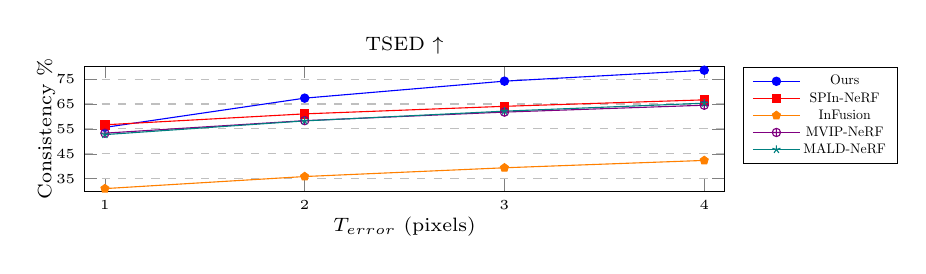
\begin{tikzpicture}
    \begin{axis}[
        title style={align=center, font=\scriptsize, yshift=-.5em},
        title={TSED $\uparrow$},
        xlabel={$T_\text{error}$ (pixels)},
        ylabel={Consistency \%},
        xmin=0.9, xmax=4.1,
        ymin=30, ymax=80,
        xtick={1,2,3,4},
        ytick={35,45,55,65,75},
        legend pos=outer north east,
        legend style={nodes={scale=0.5, transform shape}},
        label style={font=\scriptsize},
        tick label style={font=\tiny},
        ymajorgrids=true,
        grid style=dashed,
        xlabel style={yshift=1ex},
        ylabel style={yshift=-1.5ex},
        mark size=1.5pt,x
    ]
        \addplot[color=blue,mark=*,] coordinates {
        (1.0,55.6154)(2.0,67.3590)(3.0,74.1795)(4.0,78.5801)
        };
        \addplot[color=red,mark=square*,] coordinates {
        (1.0,56.6538)(2.0,61.0449)(3.0,64.0769)(4.0,66.6731)
        };
        \addplot[color=orange,mark=pentagon*,] coordinates {
        (1.0,31.0385)(2.0,35.8846)(3.0,39.3974)(4.0,42.3558)
        };
        \addplot[color=violet,mark=oplus,] coordinates {
        (1.0,53.2949)(2.0,58.3269)(3.0,61.7564)(4.0,64.5192)
        };
        \addplot[color=teal,mark=star,] coordinates {
        (1.0,52.7179)(2.0,58.2179)(3.0,62.1367)(4.0,65.3333)
        };
        \legend{Ours ,SPIn-NeRF ,InFusion ,MVIP-NeRF ,MALD-NeRF}
    \end{axis}
\end{tikzpicture}

    \end{subfigure}
    \vspace{-0.4in}
    \caption{
    Evaluation of 3D consistency of the object removal task on the SPIn-NeRF dataset using TSED.
    }
    \label{fig:tsed-spinnerf}
\end{figure}

Figures \ref{fig:tsed-spinnerf}, \ref{fig:tsed-nerfiller}, and \ref{fig:tsed-few-view}
provide a comprehensive visualization of TSED results across different tasks and different values of $T_\text{error}$. In \cref{fig:tsed-spinnerf}, we observe that when $T_\text{error} = 1.0 \text{px}$, almost all other methods achieve the same consistency as us, but do not improve (increase) as much as the error threshold increases.
This is primarily because other methods enforce 3D consistency by fusing cross-view information through a 3D radiance field, resulting in blurry output renders.
Since TSED computes SIFT features, naturally fewer such features will be detected from a blurry image, damaging the TSED score. In contrast, our method produces significantly sharper images (see \cref{tab:spinnerf} for details), resulting in more detected features and thus a higher TSED.

In \cref{fig:tsed-nerfiller} (left), when we compare the datasets (i.e., source images, directly from the generative inpainter used in each method), which are used for fitting a NeRF, we observe a significant gap between NeRFiller and ours. 
This is due to our geometry-aware inpainting model,  
which is specifically trained to propagate information across views in a multiview consistent manner.
In contrast, NeRFiller uses a geometry-\textit{un}aware inpainting model, which cannot directly apply the knowledge currently encoded in the 3D scene to inform the inpainting.
Similarly, \cref{fig:tsed-nerfiller} (right) shows that fitting a NeRF on the aforementioned datasets will result in more consistent images overall, but unsurprisingly our consistently inpainted images result in more consistent NeRF renders. Finally, \cref{fig:tsed-few-view} demonstrates the success of our method on inpainting scenes with very few views. We achieve a noticeable improvement over the baselines in terms of TSED consistency, mainly due to the difficulties encountered when fitting NeRFs on very few views, which results in both inconsistency and blurriness.
Please see our webpage for an interactive visualization of SED: \href{https://geomvi.github.io}{https://geomvi.github.io}.

\begin{figure}[t]
    \centering
    \begin{subfigure}{0.34\linewidth}
        \pgfplotsset{width=1.2\linewidth,height=3.2cm,compat=1.18}
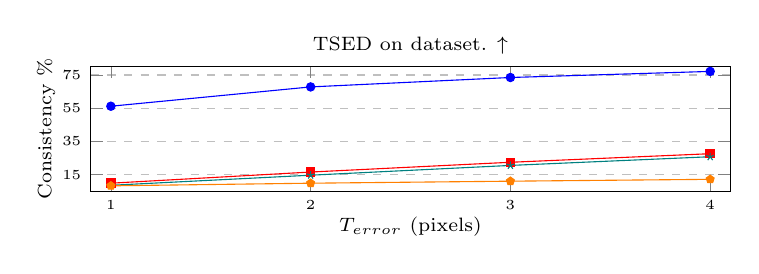
\begin{tikzpicture}
    \begin{axis}[
        title style={align=center, font=\scriptsize, yshift=-.5em},
        title={TSED on dataset. $\uparrow$},
        xlabel={$T_\text{error}$ (pixels)},
        ylabel={Consistency \%},
        xmin=0.9, xmax=4.1,
        ymin=5, ymax=80,
        xtick={1,2,3,4},
        ytick={15,35,55,75},
        legend pos=outer north east,
        legend style={nodes={scale=0.5, transform shape}},
        label style={font=\scriptsize},
        tick label style={font=\tiny},
        ymajorgrids=true,
        grid style=dashed,
        xlabel style={yshift=1ex},
        ylabel style={yshift=-1ex},
        mark size=1.5pt,x
    ]
        \addplot[color=blue,mark=*,] coordinates {
        (1.0,56.1709)(2.0,67.8006)(3.0,73.4705)(4.0,77.1361)
        };
        \addplot[color=red,mark=square*,] coordinates {
        (1.0,9.8101)(2.0,16.5348)(3.0,22.4156)(4.0,27.5712)
        };
        \addplot[color=teal,mark=star,] coordinates {
        (1.0,8.5443)(2.0,14.6361)(3.0,20.5169)(4.0,25.7516)
        }; 
        \addplot[color=orange,mark=pentagon*,] coordinates {
        (1.0,8.2278)(2.0,9.8101)(3.0,11.0232)(4.0,12.1440)
        }; 
    \end{axis}
\end{tikzpicture}

    \end{subfigure}
    \begin{subfigure}{0.60\linewidth}
        \pgfplotsset{width=0.72\linewidth,height=3.2cm,compat=1.18}
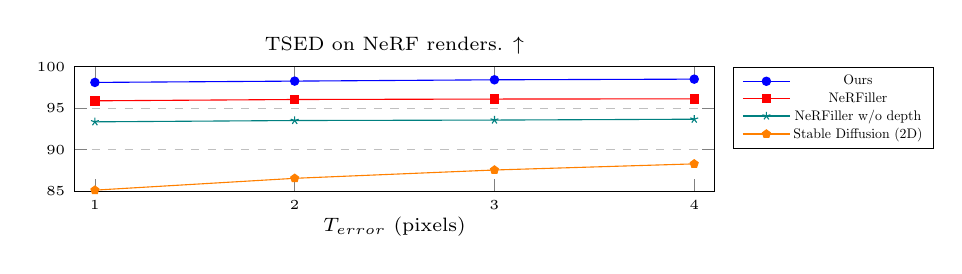
\begin{tikzpicture}
    \begin{axis}[
        title style={align=center, font=\scriptsize, yshift=-.5em},
        title={TSED on NeRF renders. $\uparrow$},
        xlabel={$T_\text{error}$ (pixels)},
        xmin=0.9, xmax=4.1,
        ymin=85, ymax=100,
        xtick={1,2,3,4},
        ytick={85,90,95,100},
        legend pos=outer north east,
        legend style={nodes={scale=0.5, transform shape}},
        label style={font=\scriptsize},
        tick label style={font=\tiny},
        ymajorgrids=true,
        grid style=dashed,
        xlabel style={yshift=1ex},
        ylabel style={yshift=-1.5ex},
        mark size=1.5pt,x
    ]
        \addplot[color=blue,mark=*,] coordinates {
        (1.0,98.1013)(2.0,98.2595)(3.0,98.4177)(4.0,98.4968)
        };
        \addplot[color=red,mark=square*,] coordinates {
        (1.0,95.8861)(2.0,96.0443)(3.0,96.0970)(4.0,96.1234)
        };
        \addplot[color=teal,mark=star,] coordinates {
        (1.0,93.3544)(2.0,93.5127)(3.0,93.5654)(4.0,93.6709)
        }; 
        \addplot[color=orange,mark=pentagon*,] coordinates {
        (1.0,85.1266)(2.0,86.5506)(3.0,87.5527)(4.0,88.2911)
        }; 
        \legend{Ours ,NeRFiller ,NeRFiller w/o depth, Stable Diffusion (2D)}
    \end{axis}
\end{tikzpicture}

    \end{subfigure}
    \vspace{-0.25in}
    \caption{
    Evaluation of 3D consistency of the scene completion task on the NeRFiller dataset using TSED. 
    The left inset shows the consistency of the ``source images'' (dataset) used to train the NeRF (i.e., the direct outputs of the generative inpainter used in each method). For NeRFiller, we use the dataset from the latest Dataset Update iteration.
    The right inset shows the consistency of the NeRF renders, from a NeRF fit to those source images.
    }
    \label{fig:tsed-nerfiller}
\end{figure}

\begin{figure}[t]
    \centering
    \begin{subfigure}{\linewidth}
        \pgfplotsset{width=0.8\linewidth,height=9em,compat=1.18}
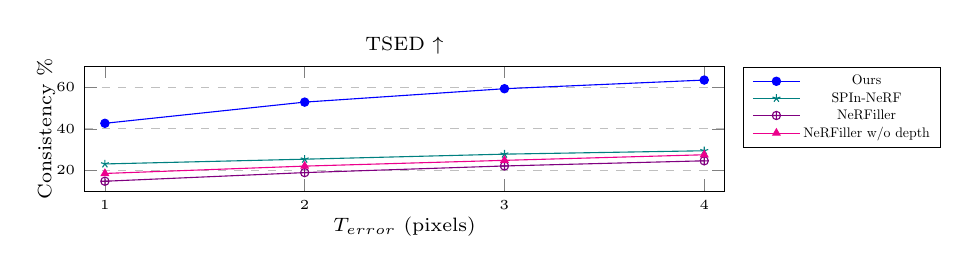
\begin{tikzpicture}
    \begin{axis}[
        title style={align=center, font=\scriptsize, yshift=-.5em},
        title={TSED $\uparrow$},
        xlabel={$T_\text{error}$ (pixels)},
        ylabel={Consistency \%},
        xmin=0.9, xmax=4.1,
        ymin=10, ymax=70,
        xtick={1,2,3,4},
        ytick={20,40,60},
        legend pos=outer north east,
        legend style={nodes={scale=0.5, transform shape}},%
        label style={font=\scriptsize},
        tick label style={font=\tiny},
        ymajorgrids=true,
        grid style=dashed,
        xlabel style={yshift=1ex},
        ylabel style={yshift=-1.5ex},
        mark size=1.5pt,x
    ]
        \addplot[color=blue,mark=*,] coordinates {
        (1.0,42.7083)(2.0,52.9167)(3.0,59.3750)(4.0,63.5417)
        };
        \addplot[color=teal,mark=star,] coordinates {
        (1.0,23.1250)(2.0,25.4167)(3.0,27.8472)(4.0,29.4792)
        };
        \addplot[color=violet,mark=oplus,] coordinates {
        (1.0,14.7917)(2.0,18.9583)(3.0,22.1528)(4.0,24.6354)
        };
        \addplot[color=magenta,mark=triangle*,] coordinates {
        (1.0,18.5417)(2.0,22.0833)(3.0,24.8611)(4.0,27.5521)
        };
        \legend{Ours
        ,SPIn-NeRF ,NeRFiller ,NeRFiller w/o depth}
    \end{axis}
\end{tikzpicture}

    \end{subfigure}
    \vspace{-0.4in}
    \caption{
    Evaluation of 3D consistency on the few-view inpainting task.
    }
    \label{fig:tsed-few-view}
\end{figure}

\section{Comprehensive Ablation Studies}
\label{supp:sec:full-ablation}

We extend the ablation studies presented in \S\ref{subsec:ablation} along three key axes: (i) comparison with the naive baseline of independent 2D inpainting, (ii) ablation of inference-time strategies, and (iii) ablating or varying various design choices in our training and fusion strategies.

\subsection{Comparison with Independent 2D inpainting}
\label{supp:subsec:independent-ablation}

\begin{table}[!t]
\centering
\tablesize
\setlength{\tabcolsep}{0.5em}
\begin{tabular}{c|ccc|cc}
Method            & PSNR $\uparrow$               & SSIM $\uparrow$              & LPIPS $\downarrow$           & MUSIQ $\uparrow$             & Corrs $\uparrow$ \\ \hline
Stable Diffusion (2D) \cite{stable.diffusion} & 24.69	          & 0.85	          & 0.10	          & 3.77	            & 1120 \\
ControlNet (2D) \cite{zhang2023controlnet}    & 21.33	          & 0.83	          & 0.14	          & 3.70	            & 1024 \\
BrushNet (2D) \cite{ju2024brushnet}           & 22.84	          & 0.83	          & 0.13	          & 3.77	            & 1081 \\
Ours                                         & \rankonecolor28.59 & \rankonecolor0.89 & \rankonecolor0.05 & \rankonecolor3.80 & \rankonecolor1250    \\
\end{tabular}
\caption{
    Evaluating our method against independent inpainting on scene completion. ``2D'' indicates independent 2D inpainting.
}
\label{tab:independent-ablation}
\end{table}

As observed in prior work \cite{weber2024nerfiller}, independent inpainting fails to produce consistent content across views.
Since \emph{reference-based geometry-awareness} is one of the core components of our approach, we also present a comparison between our geometry-aware inpainting and the naive baseline of geometry-\emph{un}aware inpainting (i.e., independent 2D inpainting), in \cref{tab:independent-ablation}.
We compare our approach to three state-of-the-art diffusion-based 2D inpainting methods: Stable Diffusion \cite{stable.diffusion} (which our model is based on), ControlNet \cite{zhang2023controlnet}, and BrushNet \cite{ju2024brushnet}.
Note that our model, just as for the 2D inpainter baselines, is also a latent diffusion model with a similar architecture, operating on a single image at a time. In other words, we do not use an explicit or implicit 3D radiance field when inpainting the views. The difference lies only in the conditioning signals: our diffusion model is informed by the 3D world and other views through the various cues passed to the generator at inference time.
After inpainting all the views, similar to our method, a NeRF is fit to the inpainted views and the rendered images and videos are assessed to compute the evaluation metrics (refer to \S\ref{subsec:eval-protocol} for details). As demonstrated, our method significantly outperforms all baselines, confirming its superior quality in the context of 3D inpainting.

\subsection{Ablation of Inference-Time Strategies}

\begin{table}[t]
\centering
\tablesize
\setlength{\tabcolsep}{0.8em}
\begin{tabular}{ccc|ccc|cc}
$\Pi$       & $D$        & St. & PSNR $\uparrow$               & SSIM $\uparrow$              & LPIPS $\downarrow$           & MUSIQ $\uparrow$             & Corrs $\uparrow$             \\ \hline
\Checkmark   & \Checkmark   & SR &                27.42 &                0.88 & 0.07                & 3.77                & 1232 \\
\XSolidBrush & \XSolidBrush & AR &                28.32 &                0.88 & \rankonecolor{0.05} & 3.78                & 1235 \\
\XSolidBrush & \Checkmark   & AR & 28.29                &                0.88 & \rankonecolor{0.05} & 3.79                & 1231 \\
\Checkmark   & \XSolidBrush & AR & \ranktwocolor{28.44} & \rankonecolor{0.89} & \rankonecolor{0.05} & \rankonecolor{3.80} & \rankonecolor{1252} \\
\Checkmark   & \Checkmark   & AR & \rankonecolor{28.59} & \rankonecolor{0.89} & \rankonecolor{0.05} & \rankonecolor{3.80} & \ranktwocolor{1250} \\
\end{tabular}%
\caption{Ablation of available inputs and inpainting strategies on the NeRFiller scenes dataset. We denote the camera parameters as $\Pi$, depth maps as $D$, inpainting strategy as St., single-reference inpainting as SR, and autoregressive inpainting as AR. Note that the last row represents our full strategy.}
\label{tab:nerfiller-ablation}
\end{table}

\begin{figure}[t]
    \centering
    \includegraphics[width=\linewidth]{figures/supp-ablation-qualitative.pdf}
    \caption{
    A qualitative example from the ablation of inference-time strategies, confirming ground-truth camera parameters and the autoregressive procedure affect the quality of the inpainted scene, whereas ground-truth depth maps have little impact.
    }
    \label{fig:ablation-qualitative}
\end{figure}

\begin{table*}[!th]
\centering
\tablesize
\begin{tabular}{ccccc|ccc|cc}
Training datasets & $\mathcal{G_\mathcal{R}}$ & Reference & Perturbation & Fusion            & PSNR $\uparrow$               & SSIM $\uparrow$              & LPIPS $\downarrow$           & MUSIQ $\uparrow$             & Corrs $\uparrow$ \\ \hline
RealEstate10K + GSO  & \XSolidBrush   & Naive                  & N/A               & Weighted average  &
24.34                & 0.85              & 0.10              & \ranktwocolor3.79              & 1113       \\
RealEstate10K + GSO  & \Checkmark     & Reprojected           & \Checkmark        & Hierarchical      &
27.12	             & 0.87	             & 0.06	             & 3.76  
                     & 1182        \\
COCO + GSO        & \XSolidBrush   & Reprojected           & \Checkmark        & Single confidence &
28.36                & 0.88              & \rankonecolor0.05 & \rankthreecolor3.78 & \ranktwocolor1223    \\
COCO + GSO        & \Checkmark     & Reprojected           & \Checkmark        & Weighted average  &
\rankonecolor29.45   & \rankonecolor0.89 & 0.06              & 3.77              & 1166    \\
COCO + GSO        & \Checkmark     & Reprojected           & \Checkmark        & Closest camera    &
27.36                & 0.88              & 0.06              & \rankthreecolor3.78 & 1204    \\
COCO + GSO        & \Checkmark     & Reprojected           & \XSolidBrush      & Hierarchical      &
\ranktwocolor29.25   & \rankonecolor0.89 & \rankonecolor0.05 & 3.72              & \rankthreecolor1222    \\
COCO + GSO        & \Checkmark     & Reprojected           & \Checkmark        & Hierarchical      &
\rankthreecolor28.59 & \rankonecolor0.89 & \rankonecolor0.05 & \rankonecolor3.80 & \rankonecolor1250    \\
\end{tabular}
\caption{Ablation of various design choices in training and fusion, including conditioning signals, datasets, and other algorithmic components. We denote the presence of geometric cues in the conditioning signals as $\mathcal{G_\mathcal{R}}$. `Closest camera' and `Weighted average' ignore the predicted confidence masks; the former solely conditions on the closest view that has been inpainted, and the latter takes a weighted average of the noise estimates, proportional to the inverse view distance between the reference view, $r$, and the target view, $t$, i.e., $\frac{1}{d((r, t))}$ (\cref{eq:view-distance}). `Single confidence' means that, since back-face and shadow masks are disabled, there is only one confidence signal, derived from the front-face mask. The last row represents our full model, which is superior on nearly all metrics, compared to other variants.
}
\label{tab:model-ablation}
\end{table*}

In \cref{tab:nerfiller-ablation}, 
we ablate various inference-time strategies of our inpainting pipeline on scene completion. 
We observe that, for wide-baseline datasets like NeRFiller, our autoregressive procedure (\S\ref{subsec:autoregressive}) is essential, as a single reference lacks sufficient information for a wide baseline (first row).
We also find that providing \duster with ground-truth depth maps has little effect on performance, highlighting the robustness of our method. However, ground-truth camera parameters have a more significant impact (second to fourth rows). This is mainly because optimizing camera parameters in \duster involves complex global alignment, whereas, when camera parameters are known, optimizing the depth maps becomes a much simpler task.
The qualitative example in \cref{fig:ablation-qualitative} also confirms our findings.

\subsection{Model Design Ablation}

Finally, we ablate or vary several design decisions in our training and fusion strategies, including training datasets, availability of geometric cues ($\mathcal{G_\mathcal{R}}$) in the conditioning signals, whether to align the reference images to the coordinate of the target image by reprojection, and whether to use mesh perturbation. According to \cref{tab:model-ablation}, we find that although mesh perturbation (\S\ref{subsec:inptrain}) does not improve image-based metrics, it has a significant impact on video-based metrics, i.e., a higher image quality and consistency.

Moreover, we find that it is essential to use our hierarchical fusion method (\S\ref{subsubsec:geo-aware-inpainting}), as alternative approaches such as ``weighted average'' and ``closest camera'' lead to lower performance. On the other hand, ``weighted average'' achieves the highest PSNR and SSIM among all settings. 
This is primarily because averaging multiple noise estimates may fuse inconsistent information, producing a blur artifact similar to NeRF renders. Since the inpainted images are already significantly blurred, fitting a NeRF does not introduce additional blurriness. This will result in higher consistency between the inpainted images and their corresponding NeRF renders, leading to higher PSNR and SSIM, though at the cost of lower overall image quality, as reflected in other metrics.

We also observe the importance of conditioning the inpainter on the geometric cues (\S\ref{subsubsec:cond-inp}).
Note that in this case, fusion is performed using a single confidence mask; with back-face and shadow masks disabled, the only confidence signal comes from the front-face mask.

As mentioned in \S\ref{subsec:inptrain}, we use a single-view image dataset instead of a multiview one, to ensure a greater data diversity. To explore the effectiveness of a single-view dataset, we compare our base model with the same model trained on RealEstate10K \cite{realestate10k} instead of COCO \cite{coco.dataset}. 
RealEstate10K, which includes a large set of scenes represented as posed multiview image sets, is commonly used for training large-scale cross-dataset novel view synthesis models (e.g., \cite{wang2021ibrnet,yu2024polyoculus}). 
To obtain multiview depth maps for RealEstate10K, we run \duster on all the videos as a pre-processing stage. \cref{tab:model-ablation} shows that our base model outperforms the one trained on RealEstate10K.

Finally, we evaluate a model naively conditioned on the reference image without any 3D reprojection, instead of our coordinate-aligned conditional inpainting. As reference-based photometric and geometric cues are synthesized for a single-view image dataset like COCO, and no actual reference image exists, we train this model on RealEstate10K.
In other words, for naive conditioning,
we must use a dataset with multiple posed views per scene,
so that one may be used as target and the other as conditioning;
our synthetic single-image reprojections, which have only one frame, therefore cannot be used. 
As presented in \cref{tab:model-ablation} (last two rows), coordinate-aligned conditional inpainting outperforms naive conditioning on RealEstate10K.

\section{Limitations}
\label{supp:sec:limitations}

While we have demonstrated improved image quality and cross-view consistency over existing baselines, in addition to applicability to the few-view scenario, some shortcomings remain in our approach. Our method relies on two external tools, Stable Diffusion \cite{stable.diffusion} for inpainting and \duster \cite{dust3r} for geometry estimation. Hence, errors caused by these tools (e.g., highly implausible inpaintings or errors in depth estimation) will be propagated throughout the process, resulting in degraded outcomes. In the case of extreme failure in these external tools (e.g. extreme errors in camera and depth estimation), our method is unable to recover.
For instance, consider \cref{fig:sd-limitation}, showing the \emph{initial} view for inpainting the ``office'' scene from the NeRFiller dataset. Clearly, the failure of our method is inherited from the Stable Diffusion inpainter, likely caused by out-of-distribution conditioning (highly irregular inpainting mask in this case). Nevertheless, our method does not catastrophically fail in such cases, even as extreme as this one, maintaining geometry and appearance quality elsewhere in the scene.
We also expect that future improvements to the mentioned tools will also be imparted to our approach.

\begin{figure}[t]
    \centering
    \includegraphics[width=\linewidth]{figures/sd_limitation.pdf}
    \caption{Our inpainting model inherits the limitations of Stable Diffusion for inpainting.}
    \label{fig:sd-limitation}
\end{figure}

